\chapter{MapReduce}

\section{Workflow}

Figure \ref{fig:MR-workflow} shows the adopted workflow\footnote{It is not the optimal one since the same query could be executed in less than four job. The idea is to structure the workflow this way so that few different MR algorithms can be applied (e.g. filtering, projection, summarization, join). }.

\begin{figure}[H]
	\centering
	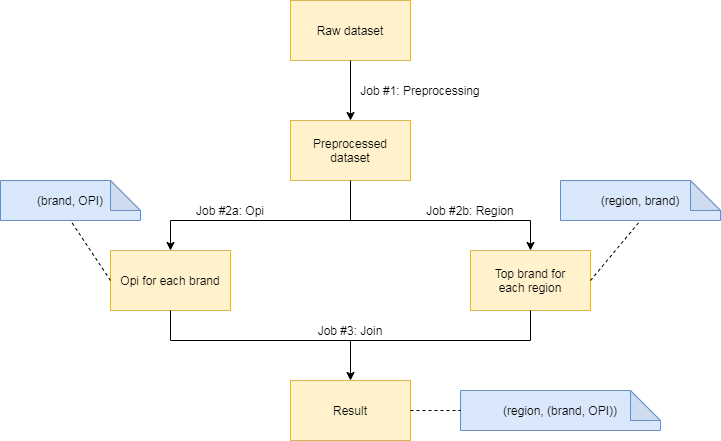
\includegraphics[scale=0.6]{images/2-mapreduce/MR-workflow.png}
	\caption{Adopted workflow for MR jobs.}
	\label{fig:MR-workflow}
\end{figure}

\section{Jobs}

\subsection{Job 1: Preprocessing}

The job executes all preprocessing operation needed to correctly use the dataset in next jobs. In particular, it fulfills the following aspects:

\begin{itemize}

  \item \textbf{Cut out header}: the raw dataset is a csv file. The header must be eliminated.
  \item \textbf{Drop useless columns}.
  \item \textbf{Drop incomplete records}: record that have missing values on mandatory fields are simply dropped. 

Job execution and interfaces are described in figure \ref{fig:MR-job-1}.
 
Raw records are read and parsed into ``Car'', i.e. custom ``Writable'' objects, during map stage. 
Each car stores data about:
\begin{itemize}
 \item Region
 \item Price
 \item Brand
 \item Fuel
 \item Odometer
\end{itemize}

The map output is a pair where the key is the default key used by Hadoop when reading text files and the value is the car itself.

The reduce stage just replaces the default key with a ``NullableWritable'' so that the whole job output is a set of records yet.

\begin{figure}[H]
	\centering
	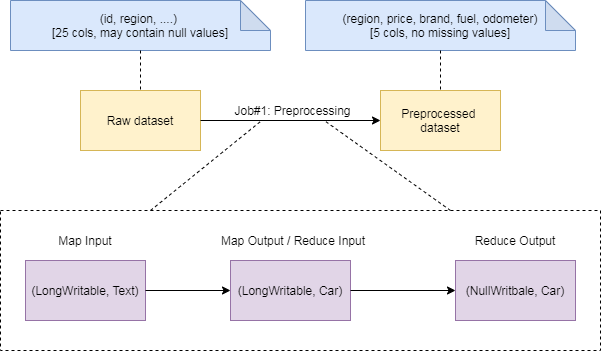
\includegraphics[scale=0.7]{images/2-mapreduce/MR-job-1.png}
	\caption{Description of ``job 1: preprocessing'' workflow and interfaces.}
	\label{fig:MR-job-1}
\end{figure}


%The dataset cardinality is reduced from 423858 to 231157.
%The dataset size is reduced from 1GB to 100MB.


\end{itemize}

\subsection{Job 2a: Opi}


\subsection{Job 2b: Region}


\subsection{Job 3: Join}


\section{Performance evaluation}
